\documentclass{report}
\usepackage{graphicx}
\usepackage[compat=1.0.0]{tikz-feynman}
\usepackage{amsmath}
\usepackage{sansmath}
\usepackage{tikz}
\usepackage{tkz-euclide}
\usepackage{tikz-3dplot}
\usepackage[makeroom]{cancel}
\usetikzlibrary{shadings,intersections,patterns}

\title{chapter10} 
\begin{document}

Problem 1. \\ \\ 
One advantage of the Lagrangian formulation is that it does not commit us to any particular coordinate system - the q's in Equation 10.6 could be Cartesian coordinates, or polar coordinates, or any other variables we might use to designate the particle's position. Suppose, for example, we want to analyze the motion of a particle that slides frictionlessly on the inside surface of a cone mounted with its axis pointing upward, as shown.\\ 
%\tdplotsetmaincoords{60}{130}

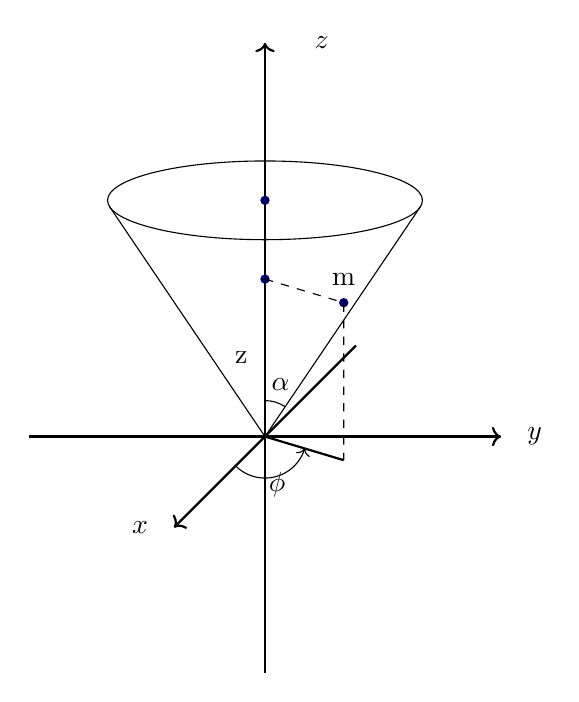
\begin{tikzpicture}
\coordinate (O) at (0,0,0);
%\tdplotsetcoord{P}{.8}{55}{60}
\draw[thick,->] (-3,0,0) -- (3,0,0) node[right =0.2]{$y$};
\draw[thick,->] (0,-3,0) -- (0,5,0) node[right= 0.5]{$z$};
\draw[thick,->] (0,0,-3) -- (0,0,3) node[left=0.2]{$x$};


\def\rx{2}    % horizontal radius of the ellipse
\def\ry{0.5}  % vertical radius of the ellipse
\def\z{3}     % distance from center of ellipse to origin
\def\p{3}  % the point on the surface
\def\pp{1.7} % the point z 
\def\ppp{1}    % the point m 
\def\ang{90}
\coordinate (p1) at (0,\p,0); 
\coordinate (p2) at (0,2,0); 
\coordinate (p3) at (\ppp,\pp,0); 
\coordinate (o) at (0,0,0);
\coordinate (y) at (0,0,1);
\coordinate (mm) at (1,-0.3,0);
\coordinate (mmm) at (1,1.5,0);
\node[fill=blue!40!black,circle,inner sep=1.2]  at (p1) {};
\node[fill=blue!40!black,circle,inner sep=1.2] (p2') at (p2) {};
\node[fill=blue!40!black,circle,inner sep=1.2] (p3') at (p3) {};
\node[above =0.1] at (p3') {m};
\node[left =0.1] at (0,1,0) {z};
\path[name path=ellipse] (0,\z) ellipse ({\rx} and {\ry});
\path[name path=horizontal] (-\rx,\z-\ry*\ry/\z) -- (\rx,\z-\ry*\ry/\z);
\path [name intersections={of = ellipse and horizontal}];
\draw[dashed] (0,2,0) -- (1,1.7,0) -- (1,-0.3,0);
\draw (intersection-1) -- (0,0) -- (intersection-2);
\draw (0,\z) ellipse ({\rx} and {\ry}); 
\draw[-,thick] (0,0,0)  -- (1,-0.3,0);
\draw pic[->,"$\phi$",draw=black,angle radius=15,angle eccentricity=1.2] {angle=y--o--mm};
%\draw pic[-,"$\alpha$",draw=black,angle radius=10,angle eccentricity=1.2] {angle=p2--o--mmm};
\draw pic[-,"$\alpha$",draw=black,angle radius=13,angle eccentricity=1.5] {angle=mmm--o--p2};
\end{tikzpicture}\\
(a) Express T and U in terms of the variables z and $\phi$ and the constants $\alpha$ (the opening angle of the cone), m(the mass of. he particle), and g (the acceleration of gravity).\\
(b) Construct the Lagrangian, and apply the Euler-Lagrangian equation to obtain differential equations for z(t) and $\phi$(t).\\
(c) Show that L = \((m\tan^{2}\alpha)z^2\phi \) is a constant of the motion. What is this quantity, physically?\\
(d) Use the result in (c) to eliminate $\phi$ from the z equation. ( You are left with a second-order differential equation for z(t); if you want to pursue the problem further, it is easiest to invoke conservation of energy, which yields a first-order equation for z.)\\

Solution\\
(a)\\
Q. How can I get the equation of motion? \\  
A. Need the velocity. \\
v = r $\dot{\phi}$ + $\dot{r}$$\phi$ \\
r = z $\tan$ $\alpha$, \\ 
so,\\
v = z $\tan$ $\alpha$ $\dot{\phi}$ + $\dot{z}$ $\tan$ $\alpha$ $\phi$ + \(\cancel{z \sec^2\alpha\dot{\alpha}}\)  \\
so, \\
\[T = \frac{1}{2}m (\tan\alpha)^2 (z^2 \dot{\phi}^2 + \dot{z}^2 \phi^2) \]
\[V = m g z\] \\ \\
(b) L = T - V \\ 
And Euler-Lagrangian equation is, \[ \frac{\partial L}{\partial q} - \frac{d}{dt} (\frac{\partial L}{\partial{\dot{q}}}) = 0 \]. \\ 
\((\frac{m\tan^2\alpha }{2}) ( \frac{\partial (z^2 \dot{\phi}^2 + \dot{z}^2 \phi^2)}{\partial z } + \frac{\partial (z^2 \dot{\phi}^2 + \dot{z}^2 \phi^2)}{\partial \phi } - \frac{d}{dt}(\frac{\partial (z^2 \dot{\phi}^2 + \dot{z}^2 \phi^2)}{\partial \dot{z}})- \frac{d}{dt}(\frac{\partial (z^2 \dot{\phi}^2 + \dot{z}^2 \phi^2)}{\partial \dot{\phi}})) - \frac{\partial(mgz)}{\partial{z}} + \frac{d}{dt}(\frac{\partial (mgz)}{\partial \dot{z}})= 0  \) \\
for z, \((\frac{m\tan^2\alpha }{2}) ( 2z\dot{\phi}^2 - 2\ddot{z}\phi^2 - 2\dot{z}2\phi\dot{\phi}) - mg = 0 \) \\
for $\phi$, \((\frac{m\tan^2\alpha }{2}) (2\phi\dot{z}^2 - 2\ddot{\phi}z^2 - 2z\dot{z}2\dot{\phi} ) = 0 \) \\

Problem 2. \\
Derive Equation 10.17 \\\\
Solution \\
Equation 10.17 \[ \frac{\partial L}{\partial A_\nu} = \frac{1}{4\pi} (\frac{mc}{\hbar})^2 A^\nu \]
The Proca Lagrangian for a Vector (Spin-1) Field ($A^\mu$). 
\[ L = \frac{-1}{16\pi} (\partial^{\mu}A^{\nu} - \partial^{\nu} A^{\mu}) (\partial_{\mu}A_{\nu} - \partial_{\nu} A_{\mu}) + \frac{1}{8\pi}(\frac{mc}{\hbar})^2 A^\nu A_\mu \ \ \ \ \ (10.16)\]\\

Note for myself\\\\
From (7.71)\\
\[F^{\mu\nu} = \begin{bmatrix}
0 & -E_x & -E_y & -E_z \\
E_x & 0 & -B_z & B_y \\
E_y & B_z & 0 & -B_x \\
E_z & -B_y & B_x & 0 
\end{bmatrix} \] \\ \\ \\ \\
From wiki - electromagnetic tensor \\ 
F = dA. where F is the electromagnetic tensor, defined as exterior derivative of the electromagnetic four-potential, A, a differential 1-form.\\
F is an antisymmetric rank-2 tensor field.\\
\(F_{\mu\nu} = \partial_\mu A_\nu - \partial_\nu A_\mu.\) \\ 
where $\partial$ is the four--gradient and A is the four-potential. \\
This is the contravariant matrix form.\\
\(F^{\mu\nu} = \begin{bmatrix}
0 & -E_x & -E_y & -E_z \\
E_x & 0 & -B_z & B_y \\
E_y & B_z & 0 & -B_x \\
E_z & -B_y & B_x & 0 
\end{bmatrix} \) \\
This is the covariant matrix form. \\
\(F_{\mu\nu} = \eta_{\alpha \nu} F^{\beta \alpha} \eta_{\mu\beta} = \begin{bmatrix}
0 & E_x & E_y & E_z \\
-E_x & 0 & -B_z & B_y \\
-E_y & B_z & 0 & -B_x \\
-E_z & -B_y & B_x & 0 
\end{bmatrix} \) \\

Q. The matrix notation for the contravariant or covariant tenstors? \\\\\
A. convention :\\
A contravariant vector : \[ v^\alpha = \begin{bmatrix}
v^0 \\
v^1 \\
v^2 
\end{bmatrix} \] 
A covariant vector : \[ u_\alpha = \begin{bmatrix}
v_0, v_1, v_2  \end{bmatrix} \]
\(\textnormal{ref: https://bjlkeng.io/posts/tensors-tensors-tensors/} \) \\  
$\mathbf{u} \cdot \mathbf{v}$ = $\sum_{i=1}^{n} u_i v_i$\\
$\mathbf{u} \cdot \mathbf{v}$ = $g(\mathbf{u},\mathbf{v})$= $g_{ij}u^i v^j$ = \( [ u^0, u^1 ] \begin{bmatrix}
 1 & 0\\
 0 & 1 
 \end{bmatrix} \begin{bmatrix} 
 v^0 \\
 v^1
 \end{bmatrix} \) \\
Q. Why $F^{\mu\nu}$ is a square matrix? if $F^{i}$ means a column matrix? \\
A. $F^{ii}$ = $F^{1 1}$ $g_{1 1}$ + $F^{1 2}$ $g_{1 2}$? contraction is needed? not sure. \\
\textnormal{ref: https://dasublogbyprashanth.blogspot.com/2023/11/contravariant-and-covariant-objects-in.html?m=1} \\ 
\end{document}